% This is samplepaper.tex, a sample chapter demonstrating the
% LLNCS macro package for Springer Computer Science proceedings;
% Version 2.21 of 2022/01/12
%
\documentclass[runningheads]{llncs}
%
\usepackage[T1]{fontenc}
% T1 fonts will be used to generate the final print and online PDFs,
% so please use T1 fonts in your manuscript whenever possible.
% Other font encondings may result in incorrect characters.
%
\usepackage{float}
\usepackage{booktabs}
\usepackage{array}
\usepackage{makecell}
\usepackage{amssymb}
\usepackage{longtable}
\usepackage{graphicx}
\usepackage{cite}
\usepackage{tikz}
\usepackage{pgfplots}
\usepackage[left=4cm,right=4cm]{geometry}
\pgfplotsset{compat=1.18}
% Used for displaying a sample figure. If possible, figure files should
% be included in EPS format.
%
% If you use the hyperref package, please uncomment the following two lines
% to display URLs in blue roman font according to Springer's eBook style:
%\usepackage{color}
%\renewcommand\UrlFont{\color{blue}\rmfamily}
%\urlstyle{rm}
%
\begin{document}
%
\title{A Systematic Review of Physiological Monitoring and Prediction in Workers in High-Risk Construction Environments}
%
\titlerunning{Physiological Monitoring and Prediction in High-Risk Construction}
% If the paper title is too long for the running head, you can set
% an abbreviated paper title here
%
\author{No Author Given}
%
\authorrunning{No Author Given}
% Proper names are abbreviated in the header.
% If there are more than two authors, use 'et al.'.
%
\institute{No Institute Given}
%
\maketitle              % typeset the header of the contribution
%
\begin{abstract}

In high-risk work environments, such as construction, heavy industry, and emergency services, safety depends on workers maintaining energy, attention, and physical well-being, although they often do not accurately perceive their own fatigue or stress. This paper presents a systematic review of 37 studies (2020-2025) on physiological monitoring of workers using artificial intelligence to detect and predict states related to occupational safety. The results show a predominance of deep learning models, especially Bi-LSTM, combined with techniques such as XGBoost. The most commonly used signals are heart rate, heart rate variability, electrodermal activity, and temperature. The main limitations include individual differences among workers, poor generalization across contexts, and the absence of more intuitive alert systems. Overall, the study provides recommendations for developing more robust, ethical, and practically applicable monitoring systems.

\keywords{Worker Health Monitoring \and Deep Learning \and Wearable Sensors \and Occupational Safety}
\end{abstract}
%
%
%
\section{Introduction}
% The first paragraph is not indented. Describe the problem, motivation, and contributions.

In recent years, the growing complexity of work environments, especially in high-risk sectors such as industry, construction, energy, and emergency services, has reinforced the need for technological solutions oriented toward worker safety and well-being. Factors such as fatigue, stress, physiological overload, and reduced attention directly affect human performance and are associated with more accidents and critical errors. This context aligns with the transition toward Industry 5.0, which promotes a people-centered approach. As noted by Leng \cite{leng2024}, this vision emphasizes a more human, sustainable, and resilient industry, placing workers' needs and interests at the center of the production process.

In parallel, advances in wearable devices and biometric sensors have made it possible to continuously and non-invasively monitor physiological signals in real time. Smartwatches and chest straps allow the collection of data such as heart rate, respiration, and electrodermal activity, providing valuable information to infer a worker's physiological state and anticipate risk situations.

However, in high-risk environments, approaches based on isolated metrics are insufficient to capture the complexity of the human physiological state. Signal variability, the influence of external factors, and work dynamics require more integrated approaches, a challenge further compounded by the fact that workers do not always correctly identify states of fatigue or stress.

In this context, the main challenge is to combine and process physiological signals with artificial intelligence techniques for robust monitoring in real-world settings. This involves challenges such as signal selection, preprocessing, temporal segmentation, and modeling.

This work is part of the European project <REDACTED>, a project focused on transforming the construction sector through robotics, artificial intelligence, and digital twins, with the goal of promoting safe collaboration between humans and autonomous systems. It presents a systematic literature review (2020-2025), based on the PRISMA methodology \cite{page2021prisma}, aimed at consolidating the state of the art on physiological signals and artificial intelligence for monitoring workers in high-risk environments and identifying trends and future challenges.
\subsection{Objectives}

The general objective of this paper is to conduct a systematic literature review on the physiological monitoring of workers in high-risk environments, with a focus on applying artificial intelligence techniques to predict human states relevant to occupational safety. Specifically, it aims to:
\begin{enumerate}
    \item \textbf{Physiological signals:} identify the most commonly used signals for detecting stress, fatigue, and physiological overload in critical work contexts.
    \item \textbf{AI methods:} analyze machine learning and deep learning techniques applied to multimodal physiological time-series modeling.
    \item \textbf{Model evaluation:} compare modeling architectures, processing strategies, and evaluation metrics reported in the literature, considering performance, robustness, and latency.
    \item \textbf{Limitations:} systematize recurring limitations associated with physiological monitoring in real-world settings, including inter-individual variability, motion artifacts, and generalization difficulties.
    \item \textbf{Practical implications:} discuss the implications of the results for project <REDACTED>, identifying directions for the future development of worker-centered preventive monitoring systems.
\end{enumerate}

\section{Systematic Review Methodology}

%\subsection{Context and Motivation}

%The growing relevance of physiological monitoring in high-risk work environments has driven a significant amount of research in recent years. In this context, a systematic literature review was conducted to identify and analyze the most relevant scientific output on emerging technologies for physiological monitoring, with a particular focus on predicting human states through artificial intelligence and machine learning techniques, making it possible to structure the field and identify robust evidence on technologies, AI models, and implementation practices.

\subsection{Search Methodology}
To ensure the rigor and reproducibility of the study, the PRISMA (Preferred Reporting Items for Systematic Reviews and Meta-Analyses) methodology was adopted, providing a structured framework for planning, conducting, and reporting systematic reviews and ensuring transparency in the search, selection, and synthesis processes.

The review covers the period from 2020 to 2025 and includes studies with real or experimental applications of physiological monitoring using wearable sensors and predictive models. The analysis aims to identify trends, techniques, practical applications, as well as challenges and limitations reported in the literature.

%The methodological process involved defining the research questions, identifying databases, building search strategies, applying inclusion and exclusion criteria, extracting data, and synthesizing the results, making it possible to build a solid state of the art that supports the development of physiological-state prediction systems.
\subsection{Research Questions}

To guide the literature search and analysis process, research questions were defined in line with the objectives of this systematic review.

\textbf{Main question.}

\begin{itemize}
    \item QP1: What technologies and artificial intelligence models are currently used for monitoring, interpreting, and predicting the physiological state of workers or individuals in high-risk environments based on data obtained from wearable sensors?
\end{itemize}

\textbf{Secondary questions.}

\begin{itemize}
    \item QS1: Which physiological signals are most commonly collected and used in the literature to monitor human state?
    \item QS2: Which machine learning and deep learning techniques are most frequently applied to analyze and predict states such as stress, fatigue, physiological load, or attention level?
    \item QS3: Which architectures and models are used for physiological time-series analysis, and what are their main advantages and limitations?
    \item QS4: Which evaluation metrics are most commonly used to validate the performance of the proposed models?
    \item QS5: Which limitations and challenges are identified in the literature for implementing real-time human-state prediction systems?
\end{itemize}

\subsection{Databases}

To ensure a representative and methodologically consistent systematic review, three academic databases were selected for their relevance in health, biomedical engineering, and applied artificial intelligence.

\begin{table}[H]
\caption{Databases used in the systematic review}
\label{tab:bases}
\centering
\begin{tabular}{c l l}
\hline
\textbf{ID} & \textbf{Database} & \textbf{URL} \\
\hline
D1 & PubMed & \url{https://pubmed.ncbi.nlm.nih.gov} \\
D2 & IEEE Xplore & \url{https://ieeexplore.ieee.org} \\
D3 & ScienceDirect & \url{https://www.sciencedirect.com} \\
\hline
\end{tabular}
\end{table}

PubMed was included because of its relevance for physiological monitoring and biosignal studies in the health context. IEEE Xplore was selected for its strong coverage of artificial intelligence, signal processing, and real-time monitoring systems. ScienceDirect complements this set by bringing together literature on digital health, sensors, and signal analysis in high-impact journals. Together, these databases provide a balance between biomedical and technical literature appropriate for the objectives of this review.

\subsection{Search Terms}

The search terms were defined from the research questions with the aim of identifying studies on wearable-sensor-based physiological monitoring and artificial intelligence techniques for human-state interpretation and prediction. Based on the thematic scopes, search strings were built combining physiological signals, acquisition devices, AI techniques, target human states, alert mechanisms, and high-risk occupational contexts, in order to ensure comprehensive coverage of the relevant literature and an appropriate delimitation of the review scope.
\begin{table}[H]
\caption{Search terms by thematic scope}
\label{tab:termos}
\centering
\resizebox{\columnwidth}{!}{%
\begin{tabular}{p{3.2cm} p{9.8cm}}
\hline
\textbf{Scope} & \textbf{Search string} \\
\hline
Physiological and Cognitive Signals & ("physiological signals" OR "heart rate" OR "HRV" OR "respiration" OR "EEG") \\
Wearable Sensors & ("wearable sensors" OR "wearable devices" OR "smartwatch" OR "chest strap" OR "physiological monitoring") \\
Artificial Intelligence Techniques & ("AI" OR "artificial intelligence" OR "machine learning" OR "deep learning" OR "neural networks" OR "time series analysis" OR "digital twin") \\
Human-State Prediction & ("stress" OR "fatigue" OR "attention" OR "human state") \\
High-Risk Contexts & ("worker safety" OR "human safety" OR "workplace monitoring" OR "industrial environments") \\
\hline
\end{tabular}
}
\end{table}

\subsection{Inclusion and Exclusion Criteria}

%The selection criteria were defined to ensure coherence with the research questions and the central objective of the review. Included studies focused on wearable-sensor-based physiological monitoring and the application of artificial intelligence techniques to interpret or predict human state in risky work contexts.

Inclusion and exclusion criteria were defined as follows:

\begin{table}[H]
\caption{Inclusion criteria}
\label{tab:criteria_inclusion}
\centering
\resizebox{\columnwidth}{!}{%
\begin{tabular}{c c p{10.5cm}}
\hline
\textbf{Type} & \textbf{ID} & \textbf{Criterion} \\
\hline
I & IC1 & Studies that use physiological signals acquired through wearable sensors or devices. \\
I & IC2 & Works that apply machine learning or deep learning AI techniques for interpretation, classification, or prediction of human state. \\
I & IC3 & Studies focused on monitoring physiological states such as stress, fatigue, physiological load, or attention level. \\
I & IC4 & Investigations applied to work environments, industrial settings, high-risk contexts, or comparable scenarios with continuous monitoring. \\
I & IC5 & Studies that describe or implement communication, interface, or notification and alert systems for the end user. \\
\hline
\end{tabular}
}
\end{table}

\begin{table}[H]
\caption{Exclusion criteria}
\label{tab:criteria_exclusion}
\centering
\resizebox{\columnwidth}{!}{%
\begin{tabular}{c c p{10.5cm}}
\hline
\textbf{Type} & \textbf{ID} & \textbf{Criterion} \\
\hline
E & EC1 & Publications not written in English. \\
E & EC2 & Studies published before 2020. \\
E & EC3 & Non-peer-reviewed publications, including opinion pieces, abstracts, posters, patents, or books. \\
E & EC4 & Duplicate studies. \\
E & EC5 & Studies that do not use real physiological data or rely exclusively on simulated data without validation. \\
E & EC6 & Works focused solely on hardware or sensor design, without physiological-state analysis using AI models. \\
\hline
\end{tabular}
}
\end{table}

\subsection{PRISMA Diagram}
\label{sec:prisma}

The study selection process followed the PRISMA guidelines, ensuring transparency, reproducibility, and methodological rigor in the systematic review. The main phases of the process are summarized below.

\begin{figure}[H]
\centering
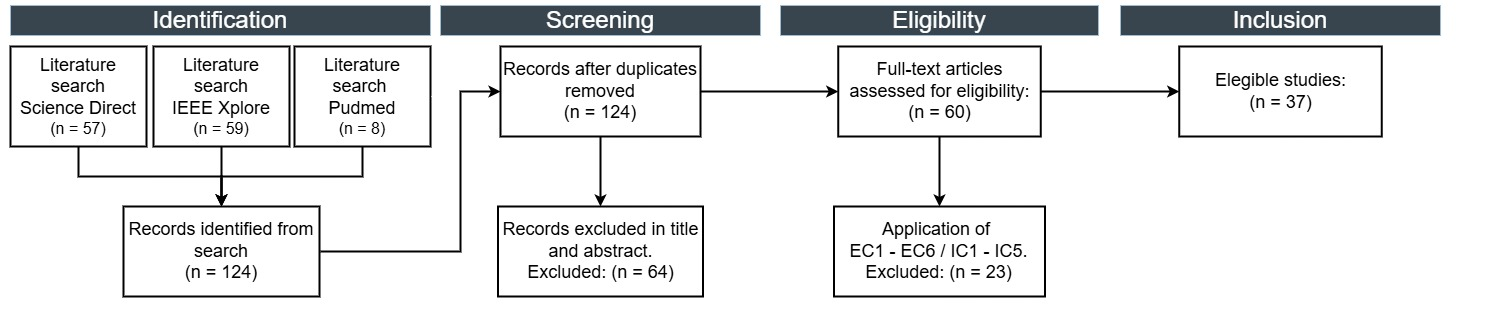
\includegraphics[,width=1\textwidth]{PRISMA.jpg}
\caption{PRISMA Diagram}
\label{fig:prisma}
\end{figure}

\textbf{Identification:} potentially relevant studies were retrieved through the search strategies applied to the selected databases, totaling 124 records (ScienceDirect: n = 57; IEEE Xplore: n = 59; PubMed: n = 8). After duplicate removal, all records were considered unique.

\textbf{Screening:} title and abstract screening led to the exclusion of 64 articles due to lack of relevance or misalignment with the review objective.

\textbf{Eligibility:} the full texts of the remaining 60 articles were assessed, and 23 studies were excluded for not meeting the defined inclusion and exclusion criteria (EC1-EC6, IC1-IC5).

\textbf{Inclusion:} finally, 37 studies were selected and included in the qualitative analysis of this systematic review.




\subsection{Quality Assessment of the Included Studies}
\label{sec:evaluacion}

To complement the systematic review, a quality assessment process was developed to apply quality criteria and prioritize the most relevant studies (Table~\ref{tab:evaluacion}), an essential step given the multidisciplinary nature of the topic.

\begin{table}[H]
\caption{Quality questions}
\label{tab:evaluacion}
\centering
\resizebox{\columnwidth}{!}{%
\begin{tabular}{l p{10cm} l}
\toprule
QA & Question & Score \\
\midrule
QA1 & The study uses physiological signals acquired through wearable sensors or devices. & Yes (+1); No (0) \\
QA2 & ML or DL AI techniques are applied for interpretation, classification, or prediction. & Yes (+1); No (0) \\
QA3 & The study monitors or predicts physiological states such as stress, fatigue, physiological load, or attention. & Yes (+1); No (0) \\
QA4 & The research applies to construction sites, high-risk environments, or comparable settings. & Yes (+1); No (0) \\
\bottomrule
\end{tabular}
}
\end{table}

Each article was evaluated across four key criteria: 1 point for affirmative answers, 0 for negative answers, and 0.5 for partial answers. This procedure made it possible to identify the works with the greatest technical affinity and guide the selection of the most relevant strategies and architectures. %the studies and their respective scores are provided in Appendix~\ref{AppendixA}, Table~\ref{tab:appendixA_single}.

To support the analysis and answer the research questions, the 12 articles that obtained the maximum score were considered. These constitute the core of the review, as they are directly aligned with the technical and contextual objectives of the work. The remaining studies are used to support contextualization and discussion.

\section{Systematic Review Results}

This section presents, in a structured manner, the results of the studies included in the systematic review, synthesizing the literature's answers to the research questions as well as the main trends, differences in approach, and relevant contributions to physiological monitoring and prediction.

\subsubsection*{QS1: Which physiological signals are most commonly collected and used in the literature for human-state monitoring?}
\label{subsec:qs1}

The scientific literature shows a clear tendency to use multimodal systems that combine several biological metrics to obtain a comprehensive view of an individual's state. Cardiovascular signals are the most recurrent indicators. Authors such as Fasoyinu et al. and Wang et al. \cite{fasoyinu2025,wang2024} highlight that heart rate (HR) and heart rate variability (HRV) are fundamental pillars for monitoring in high-risk environments such as construction. This position is supported by Thomas et al. and Sim et al.\cite{thomas2025,sim2023}, who focus on HRV specifically for stress and mental-health detection, using precise metrics such as RMSSD (Root Mean Square of Successive Differences), a statistical measure used in HRV analysis.

Electrodermal activity (EDA/GSR) emerges as the second most relevant indicator, especially in the analysis of fatigue and thermal stress. Umer et al. and Ojha et al. \cite{umer2025,ojha2024} emphasize the importance of the phasic and tonic components of EDA in assessing sympathetic nervous system activity. Morillo et al. \cite{albarran2025} also advocate the use of EDA and skin temperature as non-invasive alternatives aligned with Industry 5.0.

Regarding neuromuscular and cerebral activity, Cheng et al. and Kakhi et al. \cite{cheng2025,kakhi2025} use EEG to assess mental fatigue and accident risk, while Anjum et al. and Karim et al. \cite{anjum2025,karim2025} use sEMG for muscle-fatigue analysis.

Finally, there is a growing integration of complementary signals to improve model accuracy. Goutham et al. and Fasoyinu et al. \cite{goutham2025,fasoyinu2025} include PPG, pulse oximetry, and body temperature, while Wang et al. and Karim et al. \cite{wang2024,karim2025} incorporate behavioral metrics such as eye tracking and accelerometry data to relate physiological response, movement, and posture.

\begin{figure}[H]
\centering
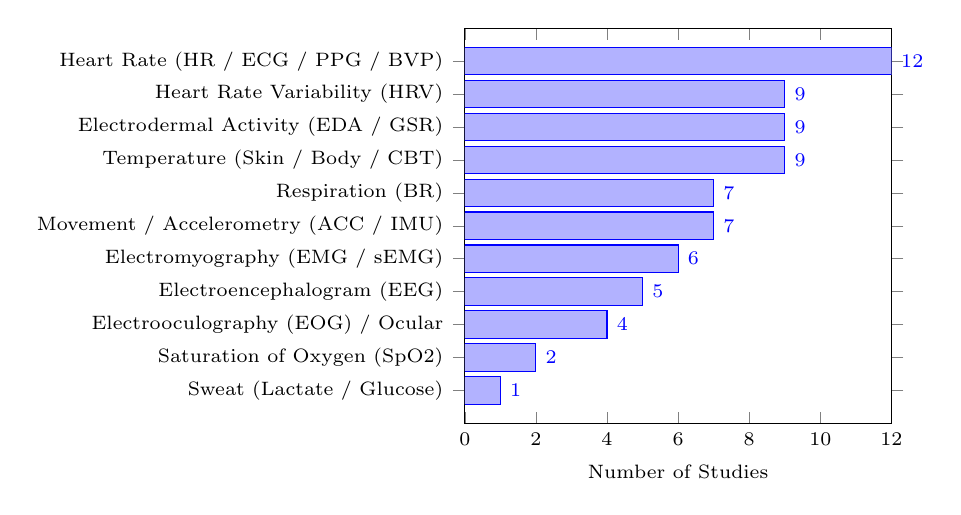
\begin{tikzpicture}
\begin{axis}[
    xbar,
    width=7cm,
    height=6.6cm,
    font=\scriptsize,
    xlabel={Number of Studies},
    ytick={1,2,3,4,5,6,7,8,9,10,11},
    yticklabels={Sweat (Lactate / Glucose),Saturation of Oxygen (SpO2),Electrooculography (EOG) / Ocular,Electroencephalogram (EEG),Electromyography (EMG / sEMG),Movement / Accelerometry (ACC / IMU),Respiration (BR),Temperature (Skin / Body / CBT),Electrodermal Activity (EDA / GSR),Heart Rate Variability (HRV),Heart Rate (HR / ECG / PPG / BVP)},
    yticklabel style={rotate=0,anchor=east},
    nodes near coords,
    enlarge y limits=0.1,
    bar width=0.35cm,
    xmin=0,
    xmax=12,
]
\addplot coordinates {(1,1) (2,2) (4,3) (5,4) (6,5) (7,6) (7,7) (9,8) (9,9) (9,10) (12,11)};
\end{axis}
\end{tikzpicture}
\caption{Frequency of Use of Physiological Signals}
\label{fig:sinais}
\end{figure}

Figure~\ref{fig:sinais} shows the distribution of physiological signals used in the 12 analyzed studies for detecting fatigue, stress, and overload in high-risk work environments. Heart rate is the most used signal (12/12), followed by heart rate variability (HRV) (9/12), electrodermal activity (EDA/GSR) (9/12), and temperature (9/12), all associated with monitoring physical, mental, and thermal load.

Signals such as movement and accelerometry (7/12), respiration (7/12), and electromyography (EMG) (6/12) are used to characterize physical activity and muscle fatigue. Finally, EEG (5/12) and ocular metrics (4/12) are used to assess cognitive load and vigilance, while SpO2 and sweat biomarkers appear more sporadically as complementary indicators.

\subsubsection*{QS2: Which machine learning and deep learning techniques are applied to the analysis and prediction of human states?}
\label{subsec:qs2}

The analyzed literature shows a strong convergence toward the use of artificial intelligence for interpreting physiological data, divided between classical Machine Learning (ML) and Deep Learning (DL) methods.

In classical ML, Thomas et al. and D. Goutham et al. \cite{thomas2025,goutham2025} highlight XGBoost as an effective model for stress and fatigue classification. In addition, Fasoyinu et al., Wang et al., and Morillo et al. \cite{fasoyinu2025,wang2024,albarran2025} report recurring use of Random Forest, SVM, and KNN for activity classification and risk detection.

In Deep Learning, Umer et al. and Karim et al. \cite{umer2025,karim2025} emphasize recurrent architectures such as LSTM, Bi-LSTM, and GRU for modeling temporal dependencies in physiological signals. In parallel, Anjum et al. and Ojha et al. \cite{anjum2025,ojha2024} use CNN and 1D-CNN, including architectures such as autoencoders and the FatigueNet model, for automatic feature extraction.

More recently, Cheng et al. \cite{cheng2025} explore graph neural networks (GNNs) combined with metaheuristic optimization, while Kakhi et al. and Ojha et al. \cite{kakhi2025,ojha2024} highlight transfer learning and domain adaptation to reduce inter-individual variability.

\begin{figure}[H]
\centering
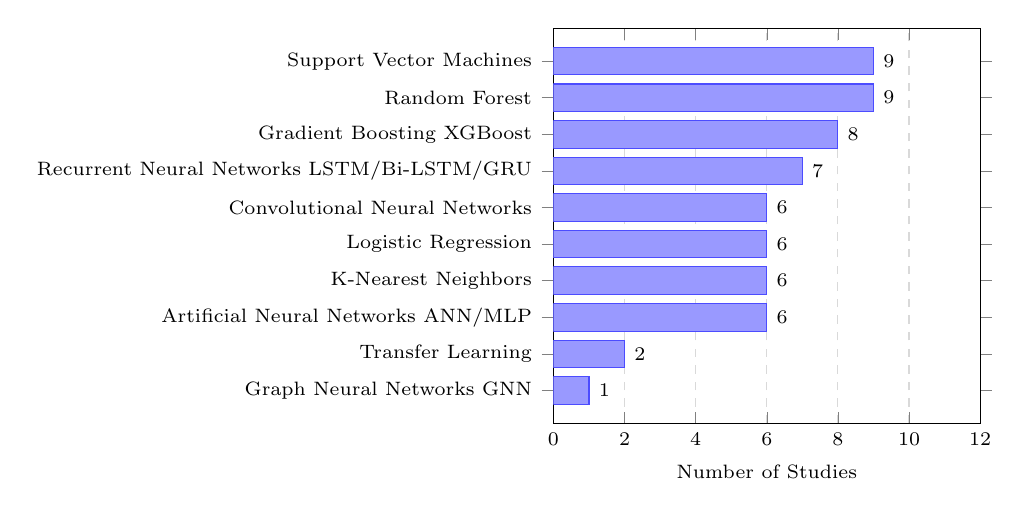
\begin{tikzpicture}
\begin{axis}[
    xbar,
    width=7cm,
    height=6.6cm,
    font=\scriptsize,
    xlabel={Number of Studies},
    symbolic y coords={
        Graph Neural Networks GNN,
        Transfer Learning,
        Artificial Neural Networks ANN/MLP,
        K-Nearest Neighbors,
        Logistic Regression,
        Convolutional Neural Networks,
        Recurrent Neural Networks LSTM/Bi-LSTM/GRU,
        Gradient Boosting XGBoost,
        Random Forest,
        Support Vector Machines
    },
    ytick=data,
    nodes near coords,
    nodes near coords align={horizontal},
    enlarge y limits=0.1,
    bar width=0.35cm,
    xmin=0,
    xmax=12,
    xmajorgrids=true,
    grid style={dashed,gray!30}
]
\addplot[fill=blue!40, draw=blue!70] coordinates {
    (1,Graph Neural Networks GNN)
    (2,Transfer Learning)
    (6,Artificial Neural Networks ANN/MLP)
    (6,K-Nearest Neighbors)
    (6,Logistic Regression)
    (6,Convolutional Neural Networks)
    (7,Recurrent Neural Networks LSTM/Bi-LSTM/GRU)
    (8,Gradient Boosting XGBoost)
    (9,Random Forest)
    (9,Support Vector Machines)
};
\end{axis}
\end{tikzpicture}
\caption{Frequency of Use of Machine Learning and Deep Learning Techniques}
\label{fig:tecnicas_ia}
\end{figure}

Figure~\ref{fig:tecnicas_ia} shows the distribution of AI techniques used in the 12 analyzed studies. Classical machine learning methods predominate, with SVM and Random Forest present in 9/12 studies and XGBoost in 8/12, due to their robustness and high accuracy on nonlinear data.

In Deep Learning, LSTM/GRU (7/12) and CNN (6/12) are widely used in physiological time-series analysis. Simpler methods such as Logistic Regression and KNN (6/12) remain relevant because of their interpretability.

Finally, Transfer Learning (2/12) emerges as an approach for adapting to new users, while GNNs (1/12) are applied in hybrid models to capture complex relationships between temporal and static variables, improving critical risk detection.

\subsubsection*{QS3: Which architectures and models are used for physiological time-series analysis, and what are their main advantages and limitations?}
\label{subsec:qs3}

Physiological time-series analysis requires architectures capable of handling the sequential and dynamic nature of the data. In the literature, Recurrent Neural Networks (RNNs), particularly LSTM and GRU, are the most used approaches. Umer et al. and Fasoyinu et al.\cite{umer2025,fasoyinu2025} emphasize their ability to mitigate the vanishing-gradient problem, allowing long-term dependencies to be captured. Within this group, Wang et al. and Karim et al.\cite{wang2024,karim2025} indicate that Bi-LSTM achieves higher accuracy (up to 98.5\%) thanks to bidirectional processing of the temporal signal.

In parallel, Convolutional Neural Networks (CNNs) have been adapted to detect morphological patterns in physiological signals. Anjum et al. propose the FatigueNet model, highlighting its robustness to heterogeneous data and lower tendency to overfit\cite{anjum2025}. More recently, hybrid approaches have gained relevance: Cheng et al.\cite{cheng2025} present the SOS-NN-GNN model, in which neural networks, GNNs, and the SOS algorithm are combined to integrate static and sequential data, enabling the capture of spatiotemporal dependencies more complex than those modeled by traditional approaches.

For tree-based models, D. Goutham et al. and Thomas et al.\cite{goutham2025,thomas2025} highlight XGBoost and LightGBM for their efficiency, scalability, and speed, with LightGBM being particularly suitable for real-time applications due to its lower memory consumption. Sim et al.\cite{sim2023} add that implementing these models in edge computing, with quantization techniques, reduces latency and enhances data privacy.

Despite these advances, important limitations remain. Kakhi et al. and Ojha et al.\cite{kakhi2025,ojha2024} emphasize the low interpretability of deep learning models. Wang et al.\cite{wang2024} note sensitivity to motion artifacts in physiological signals. Morillo et al. and Anjum et al.\cite{albarran2025,anjum2025} also point to generalization problems in real-world contexts.

\subsubsection*{QS4: Which evaluation metrics are most commonly used to validate the performance of the proposed models?}
\label{subsec:qs4}

Validation of artificial intelligence models in physiological monitoring is based on multiple metrics that assess performance from different perspectives. Consistently, Fasoyinu et al., Wang et al., and Cheng et al.\cite{fasoyinu2025,wang2024,cheng2025} use Accuracy as the main metric, complemented by F1-score and AUC-ROC due to the typical class imbalance in physiological data.

D. Goutham et al. and Morillo et al.\cite{goutham2025,albarran2025} place special emphasis on F1-score and Recall to ensure the detection of critical states, with Morillo et al. reinforcing statistical robustness through weighted F1 and bootstrap confidence intervals. Umer et al. and Anjum et al.\cite{umer2025,anjum2025} complement the evaluation with confusion matrices to analyze classification errors between fatigue levels.

In regression tasks, Karim et al., Kakhi et al., and Fasoyinu et al.\cite{karim2025,kakhi2025,fasoyinu2025} use RMSE and MAE to measure the error between predictions and real physiological values.

Finally, Ojha et al.\cite{ojha2024} introduce consistency metrics such as KL divergence and accuracy variability to assess generalization across subjects, which are crucial in heterogeneous real-world settings.

\subsubsection*{QS5: Which limitations and challenges are identified in the literature for implementing real-time human-state prediction systems?}
\label{subsec:qs5}
At the technical and operational level, Wang et al. and Kakhi et al.\cite{wang2024,kakhi2025} highlight latency and network instability problems in construction environments. Sim et al. and Umer et al.\cite{sim2023,umer2025} refer to limitations of edge computing, especially in terms of memory, processing, and energy autonomy. Fasoyinu et al.\cite{fasoyinu2025} also add hardware fragility under adverse conditions.

Regarding data quality, Ojha et al. and Wang et al.\cite{ojha2024,wang2024} identify motion artifacts as the main source of signal degradation. Anjum et al. and Ojha et al.\cite{anjum2025,ojha2024} also highlight the domain shift problem, caused by variability across individuals, which limits model generalization.

At the human and ethical level, Fasoyinu et al. and Karim et al.\cite{fasoyinu2025,karim2025} mention concerns about privacy and surveillance, while Wang et al.\cite{wang2024} highlight usability limitations of the devices. Umer et al. and D. Goutham et al.\cite{umer2025,goutham2025} also stress the lack of model interpretability, which reduces trust in their use in critical contexts.

\section{Discussion}

In this section, the previously presented results are interpreted from the perspective of implementation in project <REDACTED>, with a focus on the design of the physiological-monitoring module, operational viability on-site, and impact on occupational safety.

\subsubsection*{Priority physiological signals for implementation}

The results indicate a clear hierarchy of physiological signals for high-risk environments, with heart rate (HR) and heart rate variability (HRV) as the main indicators of fatigue and stress, serving as the basis for early monitoring in the context of project <REDACTED>.

Electrodermal activity (EDA) and temperature emerge as complementary signals that can increase system sensitivity in detecting critical states, especially in multimodal approaches using non-intrusive wearable sensors.

By contrast, signals such as EEG and EMG, although informative, present practical limitations in industrial environments due to their intrusiveness and sensitivity to noise, making them less suitable than wearable-device-based solutions.

\subsubsection*{Modeling strategy for the predictive module}

The results indicate that the complexity of physiological signals from wearables requires a hybrid modeling approach in the context of project <REDACTED>, combining classical machine learning and deep learning methods.

Models such as SVM and Random Forest stand out for their efficiency and low latency in resource-constrained scenarios, while architectures such as LSTM and GRU are essential for capturing temporal dynamics associated with the evolution of fatigue and stress.

In addition, variability across users reinforces the need for personalized calibration and dynamic adaptation mechanisms, enabling more continuous and accurate communication of risk levels beyond binary classifications.

\subsubsection*{Advantages and limitations of architectures in real-world settings}

The results indicate that architecture selection should consider not only accuracy in controlled settings but also suitability for the sequential nature of the data and the operational constraints of construction sites.

Recurrent models such as LSTM and Bi-LSTM stand out for capturing temporal dependencies, enabling the differentiation of short-term effort from accumulated fatigue patterns, while LightGBM and XGBoost offer practical advantages in terms of computational efficiency and real-time implementation.

Together, this evidence suggests a hybrid solution for project <REDACTED> that balances performance, latency, and operational viability, while also including robust preprocessing and validation on real data to mitigate limitations such as motion artifacts, low interpretability, and poor generalization.

\subsubsection*{Safety-oriented validation metrics}

The metric analysis indicates that Accuracy is insufficient in occupational safety contexts because of the imbalance between normal and critical states.

For project <REDACTED>, it is essential to prioritize Recall and F1-score to reduce false negatives associated with severe fatigue and acute stress, while MAE and RMSE allow assessment of the ability to predict physiological evolution.

In addition, performance stability across users should be considered a central requirement, ensuring system consistency in the face of individual variability.

\subsubsection*{Implementation barriers and mitigation}

Transferring monitoring systems from the laboratory to construction environments requires resilient infrastructure capable of handling network instability and latency.

In this context, edge computing is recommended for local fatigue-detection processing, enabling real-time alerts without continuous reliance on the cloud.

In parallel, a multimodal approach with complementary wearables is proposed, combining smartwatches and chest straps to balance versatility and accuracy in the collection of physiological signals while reducing errors associated with motion artifacts.

Finally, it is essential to incorporate user-specific adaptive calibration, dynamically adjusting risk thresholds to individual physiological variability based on historical data.

\section{Conclusions}

This systematic review synthesizes the state of the art in physiological monitoring and human-state prediction using wearable sensors and artificial intelligence, analyzing 37 studies published between 2020 and 2025.

Based on this analysis, it is concluded that, for the context of project <REDACTED>, it is essential to adopt a multimodal and hybrid approach for \textit{in situ} monitoring. This system should rely on cardiovascular signals ($HR$/$HRV$) complemented by $EDA$ and temperature, using a combination of smartwatches and chest straps to reduce motion artifacts. In terms of modeling, a staged strategy is proposed that combines classical algorithms such as $XGBoost$, suitable for \textit{edge computing} and low latency, with recurrent networks such as $Bi-LSTM$, capable of capturing the temporal evolution of fatigue. For system validation, the need to prioritize metrics sensitive to critical failures, such as \textit{Recall} and \textit{F1-score}, is emphasized, while also integrating adaptive calibration to mitigate workers' physiological variability.

These findings directly support the design of monitoring systems adapted to construction, the selection of models that balance accuracy with the constraints of edge processing, and the development of ethical solutions aligned with the GDPR and the European Union's AI Act.

Nevertheless, the main limitations identified in the literature, inter-individual variability, poor generalization, and the need for interpretability, reinforce the importance of conducting future validation in real-world scenarios and implementing continuous calibration.

In summary, although the state of the art is promising, this research shows that there is a significant opportunity to transform these theoretical advances into applied, robust, and ethical systems oriented toward safety in the construction sector.

\begin{credits}
\subsubsection{\ackname}
This research was supported by project <REDACTED>, co-financed by the European Regional Development Fund (ERDF) through the COMPETE 2030 Program, project no. <REDACTED>, and by national funds from the Portuguese Foundation for Science and Technology (FCT), under the Research and Development Unit Project <REDACTED>.
\end{credits}

% OPCIONAL: Se precisar de teoremas, definições, etc.
% \begin{theorem}
% Seu enunciado de teorema aqui.
% \end{theorem}
%
% \begin{proof}
% Sua demonstração aqui.
% \end{proof}

% Para citações, utilize: \cite{ref_key}
% Para múltiplas citações: \cite{ref1,ref2,ref3}

% OPCIONAL: Agradecimentos e interesses concorrentes
%\begin{credits}
%\subsubsection{\ackname} 
%This work was supported by [funding source] (grant number [XXX]).
%
%\subsubsection{\discintname}
%Os autores não têm interesses concorrentes a declarar que sejam relevantes para o conteúdo deste artigo.
%\end{credits}
%
% ---- Bibliography ----
%
% BibTeX users should specify bibliography style 'splncs04'.
% References will then be sorted and formatted in the correct style.
%
%
\begingroup
\makeatletter
\let\oldthebibliography\thebibliography
\let\endoldthebibliography\endthebibliography
\renewenvironment{thebibliography}[1]{%
    \oldthebibliography{#1}%
    \fontsize{8}{8.1}\selectfont
}{%
    \endoldthebibliography
}
\makeatother
\bibliographystyle{splncs04}
\bibliography{mybibliography}
\endgroup

%\appendix
%\clearpage
\section*{Appendix A. Detailed assessment of included studies}
\label{AppendixA}

\begingroup
\scriptsize
\setlength{\tabcolsep}{2pt}
\renewcommand{\arraystretch}{1.1}
\begin{center}
\begin{longtable}{p{1.5cm} p{4cm} p{2.0cm} c c c c c}
\caption{Quality assessment of the included studies}\label{tab:appendixA_single}\\
\hline
ID & Study & Authors & QA1 & QA2 & QA3 & QA4 & Total \\
\hline
\endfirsthead

\hline
ID & Study & Authors & QA1 & QA2 & QA3 & QA4 & Total \\
\hline
\endhead

\hline
\endfoot

\hline
\endlastfoot

\cite{fasoyinu2025} & Wearable sensing devices for construction safety: Research trends, applications, challenges, and future opportunities & Fasoyinu et al. & 1 & 1 & 1 & 1 & 4 \\
\cite{wang2024} & Monitoring and evaluating the status and behaviour of construction workers using wearable sensing technologies  & Wang et al. & 1 & 1 & 1 & 1 & 4 \\
\cite{anjum2025} & Generalizing fatigue prediction models for construction workers: Cross-experiment evaluation with transfer learning across thermal and load conditions & Anjum et al. & 1 & 1 & 1 & 1 & 4 \\
\cite{cheng2025} & Automated fall risk classification for construction workers using wearable devices, BIM, and optimized hybrid deep learning & Cheng et al. & 1 & 1 & 1 & 1 & 4 \\
\cite{kakhi2025} & Fatigue monitoring using wearables and AI: Trends, challenges, and future opportunities & Kakhi et al. & 1 & 1 & 1 & 1 & 4 \\
\cite{umer2025} & Deep learning-based fatigue monitoring of construction workers using physiological signals & Umer et al. & 1 & 1 & 1 & 1 & 4 \\
\cite{albarran2025} & Early detection of physical fatigue in industry using wearable sensors and contextual modeling & Morillo et al. & 1 & 1 & 1 & 1 & 4 \\

\cite{karim2025} & Advancing physical and mental fatigue analysis in construction workers: Insights, technologies, and future directions & Karim et al. & 1 & 1 & 1 & 1 & 4 \\
\cite{ojha2024} & Worker-centric heat strain analysis: Integrating physiological signals with ensemble learning and domain adaptation & Ojha et al. & 1 & 1 & 1 & 1 & 4 \\
\cite{thomas2025} & IoT Wearable Devices to Detect and Monitor Mental Health and Stress & Thomas et al. & 1 & 1 & 1 & 1 & 4 \\
\cite{goutham2025} & AI-Driven Fatigue Prediction in Healthcare Professionals Using Wearable Sensor Data and Gradient-Boosted Machine Learning Models & Goutham et al. & 1 & 1 & 1 & 1 & 4 \\
\cite{sim2023} & Exploring Edge Machine Learning-based Stress Prediction using Wearable Devices & Sim et al. & 1 & 1 & 1 & 1 & 4 \\
\cite{he2025} & Towards a nuanced classification of mental fatigue: A comprehensive review & He et al. & 1 & 1 & 1 & 0.5 & 3.5 \\
\cite{elmousalami2025} & Electroencephalography (EEG) for psychological hazards and mental health in construction safety automation & Elmousalami et al. & 1 & 0.5 & 1 & 1 & 3.5 \\
\cite{jaros2025} & Automated recognition of worker activity using machine learning and multi-sensor fusion & Jaros et al. & 1 & 1 & 0.5 & 1 & 3.5 \\

\cite{kazar2021} & Exploring the relations between the physiological factors and the likelihood of accidents on construction sites & Kazar et al. & 1 & 0.5 & 1 & 1 & 3.5 \\
\cite{singh2025} & AI-Powered Mental Health Tracking With Smartwatch Integration for Instantaneous Stress Assessment and Assistance & Singh et al. & 1 & 1 & 1 & 0.5 & 3.5 \\
\cite{mohapatra2024} & Wearable network for multilevel physical fatigue prediction in manufacturing workersn & Mohapatra et al. & 1 & 1 & 1 & 0.5 & 3.5 \\
\cite{chen2025} & Biosignal measurement for human-robot collaboration in construction & Chen et al. & 1 & 0 & 1 & 1 & 3 \\
\cite{ardecani2025} & Assessing workers’ neuro-physiological stress reSpO & Ardecani et al. & 1 & 0.5 & 1 & 0.5 & 3 \\
\cite{xianyong2025} & Wearable smart sensors integration with AI and machine learning for tracking human health & Shi et al. & 1 & 1 & 1 & 0 & 3 \\
\cite{abuwarda2022} & Wearable devices: Cross benefits from healthcare to construction & Abuwarda et al. & 1 & 0 & 1 & 1 & 3 \\
\cite{dhanasekar2025} & NeuroAdapt: A Multimodal Emotion-Cognitive-Fatigue Adaptive BCI System for Robotic Upper-Limb Rehabilitation  & Dhanasekar et al. & 1 & 1 & 1 & 0 & 3 \\

\cite{aishwarya2024} & Multi-Purpose Wearable Biofeedback Accessories - 2024 International Conference on Power, Energy, Control and Transmission Systems & Aishwarya et al. & 1 & 1 & 1 & 0 & 3 \\
\cite{kuzhaloli2025} & Wearable Tech for Mental Health Monitoring Real-Time Stress Detection Using Biometric Sensors  & Kuzhaloli et al. & 1 & 1 & 1 & 0 & 3 \\
\cite{arya2024} & Effective Driver Fatigue Management and Prevention Using Cloud-Integrated RNN Models & Arya et al. & 1 & 1 & 1 & 0 & 3 \\
\cite{subathra2025} & A Wearable Electronic Band for Stress Understanding Using Machine Learning & Subathra et al. & 1 & 1 & 1 & 0 & 3 \\
\cite{karpagam2024} & Physiological Data-Based Stress Detection: From Wrist Sensors to Cloud Computing and User Feedback Integration & Karpagam et al. & 1 & 1 & 1 & 0 & 3 \\
\cite{narayana2025} & IoT-Enabled Health Monitoring Glove with Machine Learning-Based Risk Classification & Narayana et al. & 1 & 1 & 1 & 0 & 3 \\
\cite{jayaweera2020} & An Integrated Framework for Predicting Health Based on Sensor Data Using Machine Learning  & Jayaweera et al. & 1 & 1 & 1 & 0 & 3 \\

\cite{rajas2025} & IoT-based Mental Health Monitoring with Machine Learning  & Rajas et al. & 1 & 1 & 1 & 0 & 3 \\
\cite{devi2023} & Wearable Physiological IoT System with Neural Network to Detect an Individual IT Professional’s Stress / Emotion in Working Environments & Devi et al. & 1 & 1 & 1 & 0 & 3 \\
\cite{divyabharathi2025} & An Explainable IoT-based Framework for Anomaly Detection and Emergency Decision Management in Smart Healthcare  & Divyabharathi et al. & 1 & 1 & 0.5 & 0 & 2.5 \\
\cite{kiriti2022} & Smart band for senior citizens & Kiriti et al. & 1 & 1 & 0.5 & 0 & 2.5 \\
\cite{vinusha2023} & Smartwatch-based Vomiting Sensation Detection using Heart Rate Analysis and Metaverse Integration  & Vinusha et al. & 1 & 1 & 0 & 0 & 2 \\
\cite{devi2025} & IoT intelligent watch for child safety & Devi et al. & 1 & 1 & 0 & 0 & 2 \\

\cite{sanjeevi2024} & Smart heart monitor using machine learning & Sanjeevi et al. & 1 & 1 & 0 & 0 & 2 \\

\end{longtable}
\end{center}
\endgroup




\end{document}
